
\documentclass[preprint,12pt]{elsarticle}

\usepackage[spanish]{babel}
\usepackage{amssymb}
\usepackage{graphicx}
\usepackage{lineno}
\usepackage[utf8]{inputenc}
\usepackage{url}
\usepackage{color}
\usepackage{enumerate} 
\usepackage[hidelinks]{hyperref}


\begin{document}
	
	\begin{frontmatter}
		
		
		\title{\huge Metodología Inmon vs Metodología Kimball}
		
		\author{Mamani Ayala, Brandon        (2015052715)}
		\author{Quispe Mamani, Angelo	      (2015052826)}
		\author{Vizcarra Llanque, Jhordy	      (2015052719)}
		\author{Ordoñez Quilli, Ronald          (2015052821)}
		\author{Rodriguez Mamani, Juan      (2017057862)}
		
		\address{Tacna, Perú}
		
		\begin{abstract}
			%% Text of abstract
			
The data warehouses in English take each importance day, as organizations move from schemes of only data collection to schemes of analysis of the same. However, in spite of the great diffusion of the concepts related to data warehouses, there is not too much Information available in Spanish regarding the methodologies fo implement them In this short article we will try to provide a general explanation of one of the most used methodologies, the Kimball methodology 
		\end{abstract}
\end{frontmatter}
%%

	
	%%
	%\linenumbers
	
	%% main text
	\section{Resumen}
Los almacenes de datos (data warehouses en inglés) toman cada día mayor importancia, a medida que las organizaciones pasan de esquemas de sólo recolección de datos a esquemas de análisis de los mismos. Sin embargo a pesar de la gran difusión de los conceptos relacionados con los almacenes de datos, no existe demasiada información disponible en castellano en cuanto a las metodologías para implementarlos. En este breve artículo intentaremos brindar una explicación general de una de las metodologías más usadas, la metodología de Kimball \\
	%%
	
	%%
	%\linenumbers
	
	%% main text

\section{Objetivos}

	%%
	
	%%
	%\linenumbers
	
	%% main text

\section{Marco Teorico}

\begin{enumerate}[3.1]
    \item Introduccion. \\
\\
Un almacen de datos (data warehouse, DW) segun Inmon (Inmon 02, Imhoff y Galemmo 03), es una colecci\'on de datos orientada a un determinado \'ambito (empresa, organización, etc.), integrado, no volátil y variable en el tiempo, que ayuda a la toma de decisiones en la entidad en la que se utiliza. Se trata, sobre todo, de un historial completo de la organización, más allá de la información transaccional y operacional, almacenado en una base de datos diseñada para favorecer el análisis y la divulgación eficiente de datos (especialmente con herramientas OLAP, de procesamiento analítico en línea). Por otra parte Kimball (Kimball 98) la define como “una copia de los datos transaccionales estructurados específicamente para consultas y analisis”. Actualmente uno de los mayores impedimentos para construir este tipo de almacenes de datos es la falta de conocimiento de metodologías adecuadas para su implementación, y la disciplina para cumplirlas. En este breve art\'iculo describiremos la metodología más utilizada actualmente: la metodología de Kimball.

    \item Metodologias Actuales \\
\\
 Existen muchas metodologías de diseño y construcción de DW. Cada fabricante de software de inteligencia de negocios busca imponer una metodología con sus productos. Sin embargo, se imponen entre la mayoría dos metodologías, la de Kimball y la de Inmon. Para comprender la mayor diferencia entre estas dos metodologías, debemos explicar además de la noción de DW mencionando en la introducción, la idea de Data mart. Un Data mart (Kimball et al 98) es un repositorio de información, similar a un DW, pero orientado a un área o departamento específico de la  organización (por ejemplo Compras, Ventas, RRHH, etc.), a diferencia del DW que cubre toda la organización, es decir la diferencia fundamental es su alcance.
Desde el punto de vista arquitectónico, la mayor diferencia entre los dos autores es el sentido de la construcción del DW, esto es comenzando por los Data marts o ascendente (Bottom-up, Kimball) o comenzando con todo el DW desde el principio, o descendente.
Por otra parte, la metodología de Inmon se basa en conceptos bien conocidos del diseño de bases de datos relacionales (Inmon 02, Imhoff y Galemmo 03) la metodología para la construcción de un sistema de este tipo es la habitual para construir un sistema de información, utilizando las herramientas habituales, al contrario de la de Kimball, que se basa en un modelado dimensional (no normalizado)


    \item Metodologia Inmon \\
\\
Bill Inmon ve la necesidad de transferir la información de los diferentes OLTP (Sistemas Transaccionales) de las organizaciones a un lugar centralizado donde los datos puedan ser utilizados para el analisis (sería el CIF o Corporate Information Factory).\\
 Insiste ademas en que ha de tener las siguientes características:
\begin{itemize}
		\item Orientado a temas: Los datos en la base de datos están estructurados de forma que los datos estén relacionados.
		\item Integrado: La base de datos contiene los datos de todos los sistemas operacionales de la organización, y dichos datos deben ser consistentes.
		\item No volátil: La información no se modifica ni se elimina, una vez almacenado un dato, éste se convierte en información de sólo lectura, y se mantiene para futuras consultas.
		\item Variante en el tiempo: Los datos que sufren un cambio a través del tiempo, deben ser registrados para que los informes generados reflejen esas variaciones.
\end{itemize}

La información ha de estar a los máximos niveles de detalle. Los Dw departamentales o datamarts son tratados como subconjuntos de este Dw corporativo, que son construidos para cubrir las necesidades individuales de analisis de cada departamento, y siempre a partir de este Dw Central (del que también se pueden construir los ODS ( Operational Data Stores ) o similares).\\

\begin {center}
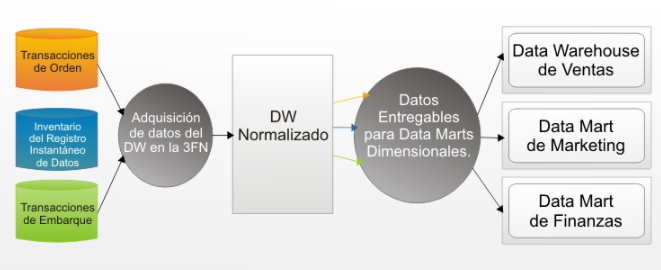
\includegraphics[scale= 0.80]{./Imagenes/inmon1.png}
\end {center}

El enfoque Inmon tambien se referencia normalmente como Top-down. Los datos son extraidos de los sistemas operacionales por los procesos ETL y cargados en las areas de stage, donde son validados y consolidados en el DW corporativo, donde ademas existen los llamados metadatos que documentan de una forma clara y precisa el contenido del DW. Una vez realizado este proceso, los procesos de refresco de los Data Mart departamentales obtienen la información de el, y con las consiguientes transformaciones, organizan los datos en las estructuras particulares requeridas por cada uno de ellos, refrescando su contenido.\\

\begin{itemize}
		\item Definición de Data Warehouse: Un Data Warehouse proporciona una visión global, común e integrada de los datos de la organización, independiente de cómo se vayan a utilizar posteriormente por los consumidores o usuarios. Normalmente en el almacén de datos habrá que guardar información histórica que cubra un amplio período de tiempo. \\
		\item Definición de Data Mart: Podemos entender un Data Mart como un subconjunto de los datos del Data Warehouse con el objetivo de responder a un determinado análisis, función o necesidad y con una población de usuarios específica. Al igual que en un data warehouse, los datos están estructurados en modelos de estrella o copo de nieve y un data mart puede ser dependiente o independiente de un data warehouse. \\
\end{itemize}



    \item Metodologia Kimball en detalle.\\
\\

La metodología se basa en lo que Kimball denomina Ciclo de Vida Dimensional del Negocio (Business Dimensional Lifecycle) (Kimball et al 98, 08, Mundy y Thornthwaite 06). Este ciclo de vida del proyecto de DW, está basado en cuatro principios básicos :
\begin{itemize}
  \item Centrarse en el negocio:  Hay que concentrarse en la identificación de los requerimientos del negocio y su valor asociado, y usar estos esfuerzos para desarrollar relaciones sólidas con el negocio, agudizando el análisis del mismo y la competencia consultiva de los implementadores.
\\
  \item Construir una infraestructura de informaci\'on adecuada: Diseña una base de información única, integrada, fácil de usar, de alto rendimiento donde se reflejará la amplia gama de requerimientos de negocio identificados en la empresa.\\
  \item Realizar entregas en incrementos significativos crear el almacén de datos (DW) en incrementos entregables en plazos de 6 a 12 meses. Hay que usa el valor de negocio de cada element identificado para determinar el orden de aplicación de los incrementos. En esto la metodología se parece a las metodologías ágiles de construcción de software.\\
  \item 
Ofrecer la solución completa proporcionar todos los elementos necesarios para entregar valor a los usuarios de negocios. Para comenzar, esto significa tener un almacén de datos sólido, bien diseñado, con calidad probada, y accesible. También se deberá entregar herramientas de consulta ad hoc, aplicaciones para informes y análisis. \\
\end{itemize} 



La construcción de una solución de DW/BI (Datawarehouse/Business Intelligence) es sumamente compleja, y Kimball nos propone una metodología que nos ayuda a simplificar esa complejidad. Las tareas de esta metodología (ciclo de vida) se muestran en la figura 1. 
De la figura 1, podemos observar dos cuestiones. Primero, hay que resaltar el rol central de la tarea de definición de requerimientos. Los requerimientos del negocio son el soporte inicial de las tareas subsiguientes. También tiene influencia en el plan de proyecto (nótese la doble fecha entre la caja de definición de requerimientos y la de planificación). En segundo lugar podemos ver tres rutas o caminos que se enfocan en tres diferentes áreas

\begin {center}
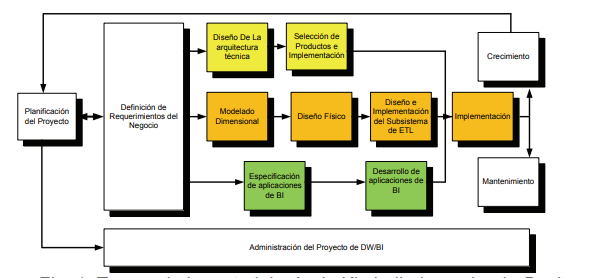
\includegraphics[scale= 0.80]{./Imagenes/1.png}
\end {center}

De la figura 1, podemos observar dos cuestiones. Primero, hay que resaltar el rol central de la tarea de definición de requerimientos.
Los requerimientos del negocio son el soporte inicial de las tareas subsiguientes. También tiene influencia en el plan de proyecto (nótese la doble fecha entre la caja de definición de requerimientos y la de planificación). En segundo lugar podemos ver tres rutas o caminos que se enfocan en tres diferentes áreas:\\

\begin{itemize}
  \item Tecnología (Camino Superior). Implica tareas relacionadas con software específico, por ejemplo, Microsoft SQL Analysis Services.
\\
  \item Datos (Camino del medio). En la misma diseñaremos e implementaremos el modelo dimensional, y desarrollaremos el subsistema de Extracción, Transformación y Carga (Extract, Transformation, and Load  ETL) para cargar el DW.
\\
  \item Aplicaciones de Inteligencia de Negocios (Camino Inferior). En esta ruta se encuentran tareas en las que diseñamos y desarrollamos las aplicaciones de negocios para los usuarios finales.
\\

\end{itemize} 
Estas rutas se combinan cuando se instala finalmente el sistema. En la parte de debajo de la figura se muestra la actividad general de administración del proyecto. A continuación describiremos cada una de las tareas. 
\end{enumerate}
\section{Proceso de Desarrollo de Modelo Kimball}
\begin{enumerate}[4.1]
 \item Planificacion del Proyecto\\

En este proceso se determina el propósito del proyecto de DW/BI, sus objetivos específicos y el alcance del mismo, los principales riesgos y una aproximación inicial a las necesidades de información.

Esta tarea incluye las siguientes acciones típicas de un plan de proyecto:


\begin{itemize}
  \item Definir el alcance (entender los requerimientos del negocio).
  \item Identificar las tareas
\item Programar las tareas
\item Planificar el uso de los recursos.
\item Asignar la carga de trabajo a los recursos
\item Elaboración de un documento final que representa un plan del proyecto.
\item Monitoreo del estado de los procesos y actividades.
\item Rastreo de problemas
\item Desarrollo de un plan de comunicación comprensiva que direccione la empresa y las áreas de TI
\end{itemize} 

\item Definicion de Requisitos de Negocios \\

La definición de requerimientos, es un proceso de entrevistar al personal de negocio y técnico, aunque siempre conviene, tener un poco de preparación previa. En esta tarea, se debe aprender sobre el negocio, los competidores, la industria y los clientes del mismo. Se debe dar una revision a todos los informes posibles de la organización; rastrear los documentos de estrategia interna; entrevistar a los empleados, analizar lo que se dice en la prensa acerca de la organización, la competencia y la industria y se deben conocer los términos y la terminología del negocio.\\
\item Modelo Dimensional \\

Es un proceso dinámico y altamente iterativo. Comienza con un modelo dimensional de alto nivel obtenido a partir de los procesos priorizados y descritos en la tarea anterior, y El proceso iterativo consiste en cuatro pasos:

\begin{itemize}
  \item Elegir el proceso de negocio
  \item Establecer el nivel de granularidad
\item  Elegir las dimensiones
\item  Identificar medidas y las tablas de hechos

\end{itemize} 

\item Diseño Fisico \\

En esta tarea, se contestan las siguientes preguntas:

\begin{itemize}
  \item ¿Cómo puede determinar cuán grande será el sistema de DW/BI?
  \item ¿Cuáles son los factores de uso que llevarán a una configuración más grande y más compleja?
  \item ¿Cómo se debe configurar el sistema?
  \item ¿Cuánta memoria y servidores se necesitan? ¿Qué tipo de almacenamiento y procesadores?
 \item ¿Cómo instalar el software en los servidores de desarrollo, prueba y producción?
 \item ¿Qué necesitan instalar los diferentes miembros del equipo de DW/BI en sus estaciones de trabajo?
 \item ¿Cómo convertir el modelo de datos lógico en un modelo de datos físicos en la base de datos relacional?
 \item ¿Cómo conseguir un plan de indexación inicial?
 \item ¿Debe usarse la partición en las tablas relacionales? 

\end{itemize} 
\item Diseño e Implementacion de Subsistema de Extraccion, Transicion y Carga \\

El subsistema de Extracción, Transformación y Carga (ETL) es la base sobre la cual se alimenta el Data warehouse. Si se diseña adecuadamente, puede extraer los datos de los sistemas de origen de datos, aplicar diferentes reglas para aumentar la calidad y consistencia de los mismos, consolidar la información proveniente de distintos sistemas, y finalmente cargar (grabar) la información en el DW en un formato acorde para la utilización por parte de las herramientas de análisis.\\

\item Mantenimiento y Crecimiento del Data Warehouse \\

Para administrar el entorno del Data Warehouse existente es importante enfocarse en los usuarios de negocio, los cuales son el motivo de su existencia, además de gestionar adecuadamente las operaciones del Data Warehouse, medir y proyectar su éxito y comunicarse constantemente con los usuarios para establecer un flujo de retroalimentación, En esto consiste el Mantenimiento. Finalmente, es importante sentar las bases para el crecimiento y evolución del Data Warehouse en donde el aspecto clave es manejar el crecimiento y evolución de forma iterativa utilizando el Ciclo de Vida propuesto, y establecer las oportunidades de crecimiento y evolución en orden por nivel prioridad.

\item Especificacion de Aplicaciones de BI \\

En está tarea se proporciona, a una gran comunidad de usuarios una forma más estructurada y por lo tanto, más fácil, de acceder al almacén de datos. Se proporciona este acceso estructurado a través de lo que llamamos, aplicaciones de inteligencia de negocios (Business Intelligence Aplications). Las aplicaciones de BI son la cara visible de la inteligencia de negocios: los informes y aplicaciones de análisis proporcionan información útil a los usuarios. Las aplicaciones de BI incluyen un amplio espectro de tipos de informes y herramientas de análisis, que van desde informes simples de formato fijo, a sofisticadas aplicaciones analíticas que usan complejos algoritmos e información del dominio. Kimball divide a estas aplicaciones en dos categorías basadas en el nivel de sofisticación, y les llama:\\

\begin{itemize}
  \item Informes Estandar\\
  \item Aplicaciones Analiticas
\\


\end{itemize} 

\item Mantenimiento y Crecimiento del Data Warehouse \\

Para administrar el entorno del Data Warehouse existente es importante enfocarse en los usuarios de negocio, los cuales son el motivo de su existencia, además de gestionar adecuadamente las operaciones del Data Warehouse, medir y proyectar su éxito y comunicarse constantemente con los usuarios para establecer un flujo de retroalimentación, En esto consiste el Mantenimiento. Finalmente, es importante sentar las bases para el crecimiento y evolución del Data Warehouse en donde el aspecto clave es manejar el crecimiento y evolución de forma iterativa utilizando el Ciclo de Vida propuesto, y establecer las oportunidades de crecimiento y evolución en orden por nivel prioridad.\\


\item Diseño y Arquitectura Tecnica \\

El área de arquitectura técnica cubre los procesos y herramientas que se aplican a los datos. En el área técnica existen dos conjuntos que tienen distintos requerimientos, brindan sus propios servicios y componentes de almacenaje de datos, por lo que se consideran cada uno aparte: El back room (habitación trasera) y el front room (habitación frontal). El back room es el responsable de la obtención y preparación de los datos, por lo que también se conoce como adquisición de datos y el front room es responsable de entregar los datos a la comunidad de usuario y también se le conoce como acceso de datos.\\
\end{enumerate}

\section{Enfoque}
 
\begin{enumerate}[5.1]
    \item Enforque Inmon. \\
\\
Para ir adentrándonos poco a poco en sus principales diferencias y poder llegar a determinar qué opción es la más adecuada en nuestros proyectos, en esta entrada expondré las características más destacadas del enfoque de Inmon.
Para él, un DataWarehouse ha de entenderse como un almacén de datos único y global para toda la empresa.\\

Un repositorio que centralice los datos de los diferentes sistemas operacionales de las organizaciones para que éstos queden validados e integrados en una única base de datos.\\

En este modelo, la premisa es que la información se almacene al máximo nivel de detalle (garantizando la futura exploración de los datos), permaneciendo invariable y no volátil, de manera que los cambios que sufran los datos a lo largo del tiempo queden registrados sin que puedan modificarse o eliminarse.\\


     \item Claves de la arquitectura \\

Estas son las claves fundamentales de la arquitectura defendida por Inmon, conocida como ‘Corporate Information Factory (CIF)’, donde el DataWarehouse centraliza todos los datos de la compañía para alimentar, a continuación, pequeños DataMarts temáticos, que serán los puntos de acceso para las herramientas de reporting. En este sentido, cada departamento tendrá su propio DataMart, abastecido con la información del DataWarehouse, listo para su análisis y explotación.

\begin {center}
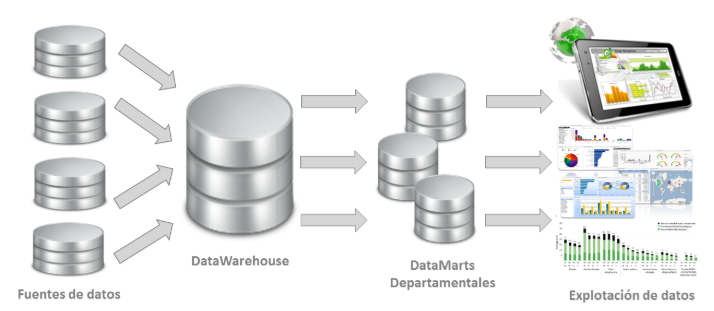
\includegraphics[scale= 1.8]{./Imagenes/img1.jpg}
\end {center}

Este enfoque de Inmon suele denominarse como una metodología de trabajo ‘Top-Down’, ya que se centra primero en una visión global de la compañía, para ir desmembrándola en pequeños sets de datos departamentales. Así, con esta arquitectura, todos los DataMarts de la organización están conectados al DataWarehouse, evitándose la aparición de incongruencias y anomalías al comparar los datos entre distintos departamentos.\\

   \item La estructura del DataWarehouse\\

En cuanto a la estructura interna del DataWarehouse, para Inmon la prioridad es que el modelo de datos esté construido en tercera forma normal. Por dar una breve explicación de lo que esto significa, el proceso de normalización consiste en aplicar una serie de reglas o normas a la hora de establecer las relaciones entre los diferentes objetos dentro de la base de datos. Con este proceso de normalización se consiguen muchos beneficios, como evitar la redundancia de los datos, mantener su integridad referencial, facilitar el mantenimiento de las tablas y disminuir el tamaño de la base de datos. Sin embargo, a diferencia de los DataWarehouse desnormalizados, las consultas exigen el empleo de queries mucho más complejas, lo que dificulta el análisis directo de la información y el uso de las herramientas de reporting. De ahí, la necesidad de construir los DataMarts que, como ya comenté, están basados en modelos dimensionales de estrella o copo de nieve, diseños fácilmente explotables por estas herramientas de análisis de datos.\\

\begin {center}
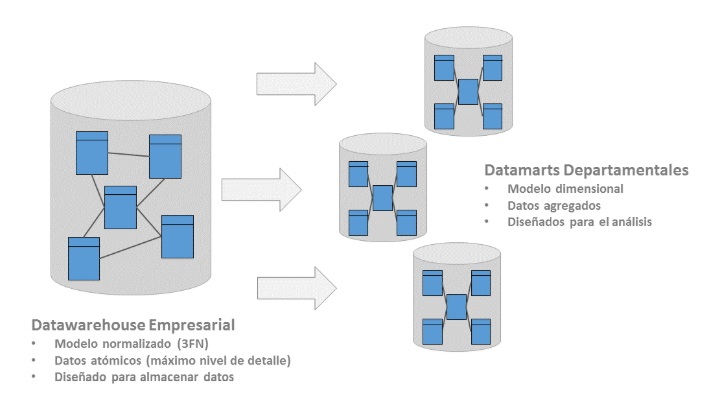
\includegraphics[scale= 1.80]{./Imagenes/img2.jpg}
\end {center}

En la próxima entrada expondré el enfoque de Ralph Kimball para, a continuación, poder hacer una comparativa de los aspectos más destacados de ambas visiones y establecer las bases para determinar que esquema se adapta más a nuestras necesidades a la hora de implantar un proyecto de Business Intelligence.

\end{enumerate}

\section{Ventajas y Desventajas}
\begin{enumerate}[5.2]
    \item Ventajas de la Metodologia Inmon.
 \\
\begin{itemize}
\item Tecnología (Camino Superior). Implica tareas relacionadas con software específico, por ejemplo, Microsoft SQL Analysis Services.
\item El almacén de datos realmente sirve como la única fuente de verdad para la empresa, ya que es la única fuente para los almacenes de datos y todos los datos en el almacén de datos están integrados.
\item Las anomalías de actualización de datos se evitan debido a una redundancia muy baja. Esto hace que el proceso ETL sea más fácil y menos propenso a fallar.
\item Los procesos de negocios se pueden entender fácilmente, ya que el modelo lógico representa las entidades de negocios detalladas.
\item Muy flexible: a medida que cambian los requisitos del negocio o cambian los datos de origen, es fácil actualizar el almacén de datos ya que una cosa está en un solo lugar.
\item Puede manejar diversas necesidades de informes en toda la empresa.
\\
\end{itemize}
 \item Desventajas de la Metodologia Inmon.
\begin{itemize}

\item El modelo y la implementación pueden volverse complejos con el tiempo, ya que involucra más tablas y combinaciones.
\item Necesita recursos que sean expertos en modelado de datos y de la propia empresa. Este tipo de recursos puede ser difícil de encontrar y, a menudo, son costosos.
\item La configuración inicial y la entrega tomarán más tiempo, y la administración debe ser consciente de esto.
\item Se necesita más trabajo de ETL ya que los almacenes de datos se crean a partir del almacén de datos.
\item Un equipo bastante grande de especialistas debe estar presente para gestionar con éxito el medio ambiente (Breslin, 2004).
\end{itemize}

 \item Ventajas de la Metodologia Kimball.
\begin{itemize}
\item Rápido de configurar y construir, y la primera fase del proyecto de almacenamiento de datos se entregará rápidamente.
\item El esquema en estrella puede ser comprendido fácilmente por los usuarios de negocios y es fácil de usar para informes. La mayoría de las herramientas de BI funcionan bien con el esquema en estrella.
\item La huella del entorno de almacenamiento de datos es pequeña, ocupa menos espacio en la base de datos y facilita la administración del sistema.
\item El rendimiento del modelo de esquema en estrella es muy bueno. El motor de la base de datos realizará una "combinación estrella" en la que se creará un producto cartesiano utilizando todos los valores de dimensión y la tabla de hechos se consultará finalmente para las filas selectivas. Se sabe que esta es una operación de base de datos muy efectiva.
\item Un pequeño equipo de desarrolladores y arquitectos es suficiente para que el almacén de datos funcione de manera efectiva (Breslin, 2004).
\item Funciona realmente bien para las métricas por departamento y el seguimiento de KPI, ya que los almacenes de datos están orientados a la información por departamento o por proceso empresarial.
\item La obtención de detalles, donde una herramienta de BI recorre varios esquemas en estrella para generar un informe, se puede lograr con éxito utilizando dimensiones conformadas.
\end{itemize}

\item Desventajas de la Metodologia Kimball.
\begin{itemize}

\item La esencia de la "fuente de la verdad" se pierde, ya que los datos no se integran completamente antes de atender las necesidades de informes.
\item Los datos redundantes pueden causar anomalías en la actualización de los datos a lo largo del tiempo.
\item Agregar columnas a la tabla de hechos puede causar problemas de rendimiento. Esto se debe a que las tablas de hecho están diseñadas para ser muy profundas. Si se agregan nuevas columnas, el tamaño de la tabla de hechos se vuelve mucho más grande y no tendrá un buen desempeño. Esto hace que el modelo dimensional sea difícil de cambiar a medida que cambian los requisitos del negocio.
\item No se pueden manejar todas las necesidades de informes de la empresa porque el modelo está orientado a los procesos de negocios en lugar de a la empresa en su conjunto.
\item La integración de datos heredados en el almacén de datos puede ser un proceso complejo.

\end{itemize}


\end{enumerate}
ETL: Este término viene de inglés de las siglas Extract-Transform-Load que significan Extraer, Transformar y Cargar. Se refiere a los datos en una empresa
\section{Diferencias}
\begin{itemize}
\item Según W. H. Inmon (considerado por muchos el padre del Data Warehouse), un Data Warehouse es un conjunto de datos orientados por temas, integrados, variantes en el tiempo y no volátiles, que tienen por objetivo dar soporte a la toma de decisiones.
\item Según Ralph Kimball (considerado el principal promotor del enfoque dimensional para el diseño de almacenes de datos), un Data Warehouse es una copia de los datos transaccionales específicamente estructurada para la consulta y el análisis.
\end{itemize}
\begin {center}
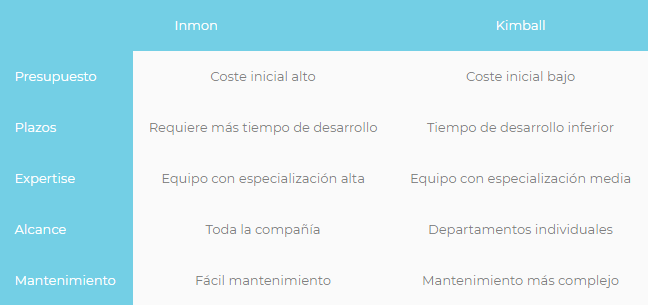
\includegraphics[scale= 0.80]{./Imagenes/vs.png}
\end {center}
\begin {center}
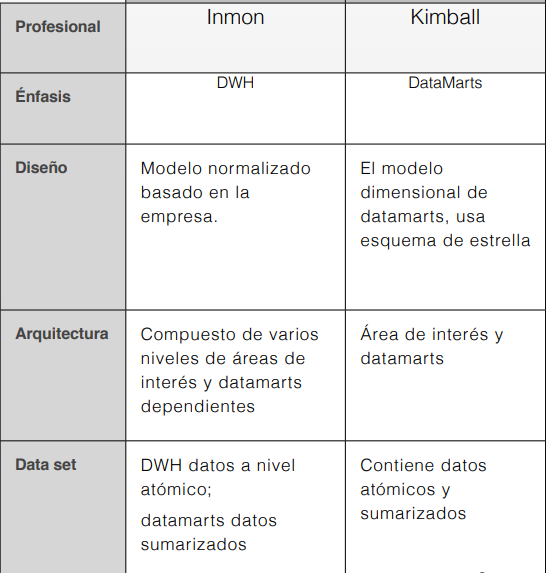
\includegraphics[scale= 0.80]{./Imagenes/vs2.png}
\end {center}
\section{Conclusion}
El método Kimball está orientado a la consulta de la información, por lo que su estructura interna está especialmente diseñada para garantizar una explotación de los datos rápida y sencilla, no requiriendo usuarios especializados para ello. Por el contrario, el método Inmon persigue la integración de todos los datos de la compañía, estando orientado hacia el almacenaje de grandes volúmenes de datos, por lo que su estructura interna normalizada se diseña para evitar la redundancia de datos, simplificar las labores de mantenimiento, etc. cuestiones que complican las consultas de la información, requiriendo que los usuarios finales estén mucho más especializados.
Así, podríamos decir que el enfoque de Kimball se ajusta más a proyectos pequeños en los que se persiga un sistema fácilmente explotable y entendible por el usuario y de rápido desarrollo, siendo el modelo de Inmon más apropiado para sistemas complejos de mayor importancia.

%%
	
	%%
	%\linenumbers
	
	%% main text

	
	
	\newpage
	
		%ESTILO
	   \bibliography{BIBLIOGRAFIA}		%ARCHIVO .bib
	   \begin{thebibliography}{0}
              \bibitem{Ronald} 
 	    \bibitem{Angelo} 
                 \bibitem{Juan} http://tdan.com/data-warehouse-design-inmon-versus-kimball/20300
                  \bibitem{Jhordy} https://blog.bi-geek.com/arquitectura-comparativa-inmon-y-kimball/
                  \bibitem{Jhordy} https://churriwifi.wordpress.com/2010/04/19/15-2-ampliacion-conceptos-del-modelado-dimensional/
                    \bibitem{Brandon} https://twooctobers.com/blog/8-data-storytelling-concepts-with-examples/
                   \bibitem{Brandon}https://www.ucasal.edu.ar/htm/ingenieria/cuadernos/archivos/5-p56-rivadera-formateado.pdf

         \end{thebibliography}
	
\end{document}

%%
%% End of file `elsarticle-template-1-num.tex'.
